\documentclass[a4paper,12pt]{article}
\usepackage[utf8]{inputenc}
\usepackage{fancyhdr}
\usepackage{enumitem}
\usepackage{hyperref}
\usepackage{natbib}
\usepackage[french]{babel}

\setlength{\parindent}{1cm}
\usepackage{mwe,lipsum}
\usepackage[section]{placeins}
\usepackage{dblfloatfix}
\usepackage{float}
\usepackage[utf8]{inputenc}
\usepackage[T1]{fontenc}
\usepackage{graphicx}
\usepackage{fullpage}
\usepackage{eso-pic}
\usepackage{layout}
\usepackage{indentfirst}
\usepackage{siunitx}
\usepackage{amsmath}
\usepackage{amssymb}
\usepackage{tabularx}
\usepackage{multicol}
\usepackage{multirow}

\usepackage{caption}
\usepackage{subcaption}

\setlength{\headsep}{0.3cm}
\renewcommand*\contentsname{Table des matières}

\begin{document}
	\pagestyle{fancy}
	\headheight=15pt
	\fancyhf{}
	\renewcommand{\footrulewidth}{0.4pt}
	
	\lhead{DNS over HTTPS}
	\rhead{IP}
	% \lfoot{Equipe 9 - 2020}
	\rfoot{\thepage}
	
	%   TITLE PAGE
	\begin{titlepage}
		
		\begin{center}
			\rule{\textwidth}{1pt} % Thick horizontal rule
			
			\vspace{2pt}\vspace{-\baselineskip} % White space between rules
			
			\rule{\textwidth}{0.4pt} % Thin horizontal rule
			
			\vspace{0.1\textheight} % White space between the top rules and title
			
			%------------------------------------------------
			%	Title
			%------------------------------------------------
			
			\textcolor{black} {
				{\Huge DNS over HTTPS}\\[0.5\baselineskip]
			}
			
			\vspace{0.01\textheight} % White space between the title and short horizontal rule
			
			\rule{0.3\textwidth}{0.4pt} % Short horizontal rule under the title
			
			\vspace{0.1\textheight}
			
			%------------------------------------------------
			%	Author
			%------------------------------------------------
			
			{\Large \textsc{Arnaud Lombardi - Théo Grosperrin}} % Author name
			
			\vspace{0.025\textheight}
			
			{\large \textsc{\today}}
			
			\vfill % White space between the author name and publisher
			
		\end{center}
		
		%------------------------------------------------
		%	Publisher
		%------------------------------------------------
		
		\centering
		{
\includegraphics[scale=0.5]{Images/INSA_LOGO.png}}\\[1.7\baselineskip]
		{
\includegraphics[scale=0.18]{Images/TC.jpg}}
		
		\vspace{0.1\textheight} % White space under the publisher text
		
		%------------------------------------------------
		%	Bottom rules
		%------------------------------------------------
		
		\centering
		
		\rule{\textwidth}{0.4pt} % Thin horizontal rule
		
		\vspace{2pt}\vspace{-\baselineskip} % White space between rules
		
		\rule{\textwidth}{1pt} % Thick horizontal rule
		
	\end{titlepage}
	
	% Front matter %
	\setcounter{page}{1}
	\pagenumbering{arabic}
	
	%------------------------------------------------
	%	Table of contents
	%------------------------------------------------
	\hspace{2cm}
	\tableofcontents
	
	\newpage
	
	\section{En quelques mots, qu'est que le DoH ?}
	Il s'agit de la résolution des requêtes DNS en utilisant le protocole HTTPS, au lieu de simples requêtes en clair sur le port 53 (DNS classique). L'objectif de cette méthode est d'augmenter la sécurité du cote utilisateur : cela permet d'améliorer la vie privée de l'utilisateur (le trafic entre le client et le serveur DNS est chiffré, illisible par les machines se trouvant sur le chemin), et d'éviter les attaques de type "man-in-the-middle".
	
	\section{Détails techniques}
	Le DoH est un standard publié par l'IETF : \href{https://tools.ietf.org/html/rfc8484}{RFC 8484}.
	
	\subsection{Le fonctionnement du DNS et ses limites}
	
	\subsection{Le fonctionnement du DoH}
	
	\section{Les différentes implémentations typiques}
	
	\subsubsection{DoH natif au sein du navigateur}
	
	C'est la méthode à privilégier, mais aussi la plus complexe à mettre en place : l'application effectue elle-même une requête DoH, elles n'ont donc pas besoin de passer par la fonction DNS du système d'exploitation. Les désavantages de cette implémentation restent multiples : l'application peut ne pas informer l'utilisateur qu'elle effectue ou non la requête de manière sécurisée (par exemple, si elle ne le supporte pas, elle n'en informera probablement pas l'utilisateur). De plus, cela demande une mise à jour de chaque application afin de la rendre compatible DoH de manière native.
	
	\begin{figure}[H]
		\begin{center}
			{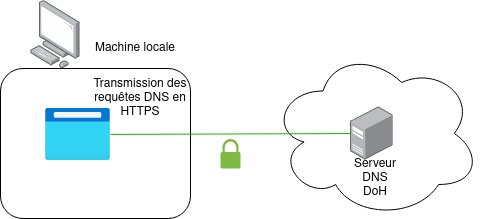
\includegraphics[scale=0.6]{Images/schema_doh_native.png}}
		\end{center}
		\caption{Schéma de l'implémentation native de DoH au sein d'une application.}
	\end{figure}
	 
	
	\subsubsection{Proxy DoH sur le réseau local}
	
	Dans ce scénario, les machines du réseau local effectuent des requêtes DNS traditionnelles sur le port 53, vers un serveur DNS installé sur le réseau local. Ce serveur DNS effectue ensuite une requête DNS récursive vers un serveur DNS compatible DoH. Ainsi, la requête est chiffrée lorsqu'elle sort du LAN.
	
	\begin{figure}[H]
		\begin{center}
			{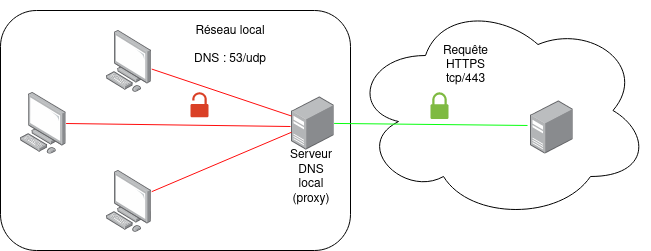
\includegraphics[scale=0.6]{Images/schema_doh_proxy_lan.png}}
		\end{center}
		\caption{Schéma de l'implémentation d'un serveur DoH proxy sur un réseau local.}
	\end{figure}
	
	On constate bien l'inconvénient de ce système : les requêtes entre les clients et le serveur local ne sont pas sécurisées, et on se base sur le fait que l'on fait confiance au serveur proxy.
	Cependant, il s'agit d'un méthode d'implémentation relativement facile à mettre en place, puisqu'elle n'implique que peu de modifications sur le réseau existant, simplement l'ajout d'un proxy sur le LAN.
	
	\subsubsection{Proxy DoH sur système local}
	
	Ici, le système est configuré pour envoyer les requêtes DNS à lui-même, puisqu'on installe un serveur proxy sur celui-ci. Ce proxy se charge d'effectuer les requêtes de manière sécurisée (donc DoH) pour chaque requête DNS classique qu'il reçoit.
	Cette méthode permet d'utiliser des applications n'implémentant pas le DoH de manière native sans compromettre la sécurité des requêtes sur le LAN. Cependant, elle est lourde puisqu'elle implique d'installer un proxy sur chaque machine.
	
	\begin{figure}[H]
		\begin{center}
			{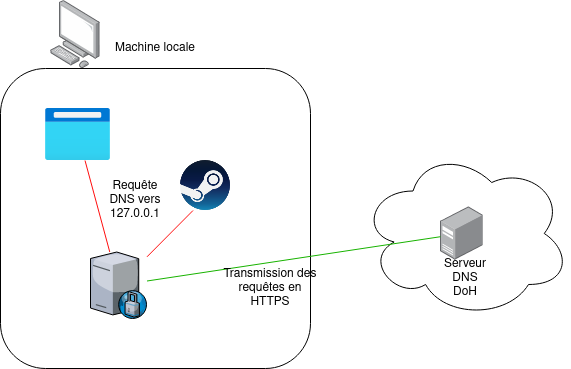
\includegraphics[scale=0.6]{Images/schema_doh_proxy_local.png}}
		\end{center}
		\caption{Schéma de l'implémentation d'un serveur proxy DoH sur le système local.}
	\end{figure}
	
	\subsubsection{Tableau récapitulatif}
	
	\section{Mise en contexte}
	
	\subsection{Support logiciel}
	
	\subsubsection{Système d'exploitation}
	
	\subsubsection{Navigateurs compatibles}
	
	\subsubsection{Serveurs compatibles}
	
	\subsection{Critiques}
	
	\section{Les problèmes que peuvent poser le DoH}
	
	
	
\end{document}